\section{Motivation} % p 2.5
    Clinical diagnostics and research has been improved dramatically with emergence of volumetric imaging such as \ac{CT} and \ac{MRI} technology which enables visualizing body parts and organs.
    Since its invention in xx, the number of acquired \ac{CT} scans has increased xx-fold until 2024. The importance of \ac{MRI} scans, which offer better soft-tissue contrast without exposing radiation to the patient examined \citep{xx}, has likewise increase with now approximately xx million scans taken every year worldwide.
    % Are there some papers that have evidence for benefit of methods?

    Volumetric imaging offers the benefit of capturing the organ of interest unaltered in \ac{3D} space. However, visualizing the \ac{3D} volume is currently still performed on \ac{2D} screens where in case of \ac{CT} and \ac{MRI} a suitable form of \ac{3D} translucent projection for the densly acquired volume has to be found or individual view planes / imaging slices have to be selected for examination. Automated processing is needed in the first case for the visualization itself and in the latter case automated processing can support clinicians navigating the \ac{3D} volume, help classifying organ boundaries, measuring tumour sizes and highlight organ deformations, all of which is complicated to perform manually when navigating a \ac{3D} volume.

    Deep learning with its basic principles invented in the last century, has become a de-facto standard now for automated processing in versatile fields such as for processing text, images, audio, video, analogous signals, biological processes and molecule configurations, agent simulations purely digitally or in combination with sensors and actuators for physical interaction \citep{xx} and has created a significant technology push throughout all of the mentioned areas of application \citep{xx}.
    Of course, this holds true for volumetric medical image analysis as well where formerly hand-crafted method design is now combined or even entirely replaced with data-driven, learning-based methods \citep{xx}.

    Deep learning as a special concept of artificial learning, was sought to mimick the neuronal activity in brain tissue and it has been found that higher-level concepts of human learning such as reasoning about generalization applies to deep learning in similar ways \citep{xx}. Now a question is raised to the reader:

    \begin{quote}
        \centering \Large
        Which elements are needed for \emph{generalization?}
        % $\vdots$
    \end{quote}

    \begin{figure}
        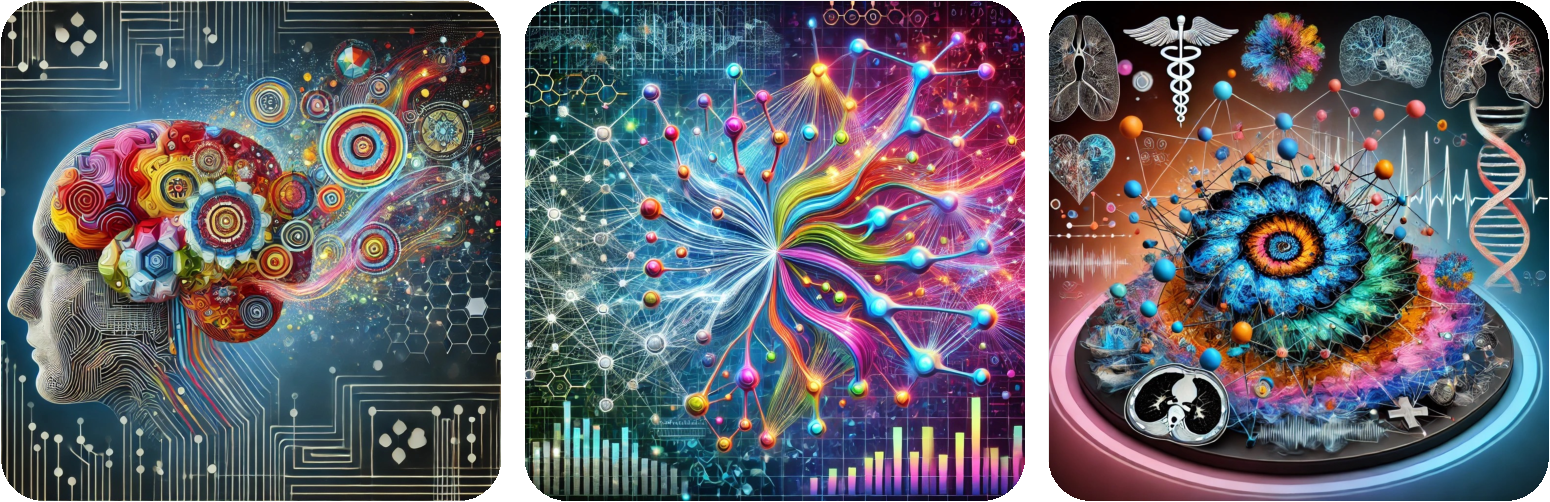
\includegraphics[width=\textwidth]{sections/01_introduction/figures/synthesized_generalization.pdf}
        \caption{Visualizations of a state-of-the-art text-to-image generator DALL$\cdot$E 3 \citep{xx} when prompted to \textquote{visualize generalization} (left), to \textquote{visualize generalization in deep learning} (middle) and to \textquote{visualize generalization in deep learning for volumetric medical images} (right).}
        \label{fig:synthesized_generalization}
    \end{figure}

    % This question will serve us as starting point to motivate the main aspects of this thesis.
    As a help for brainstorming, a deep learning-based text-to-image generator \citep{xx} was prompted to visualize \textquote{generalization}, \textquote{generalization in deep learning} and \textquote{generalization for volumetric medical images} in \figref{fig:synthesized_generalization}.

    \textquote{Generalization} (\figref{fig:synthesized_generalization}, left) was depicted as a human brain related topic, showing abstract organic shapes emerging from the central skull boundary.
    % as well as regular wire-like structures at the top and bottom of the image.
    The initial definition of generalization is indeed brain related and was described for fear learning, where two sub-mechanisms of conditioned learning --- generalization and specialization --- were discovered \citep{xx, banich2011generalization}. % TODO primary source needed
    In fear learning, initially an instance-based generalization\footnote{Opposed to the presented finding, in deep learning, specialization is considered to be formed instance-based} occurs that maps a novel fear to an environment \citep{banich2011generalization}. Later, this generalization is specialized and mapped to specific environmental stimuli leading to the learning of discriminative aspects \citep{banich2011generalization}.
    Learning (of generalization) on the cell level, is assumed to work as the change of neuron connection-strength through synaptic plasticity \citep{do1949organization,martin2000synaptic}. The visualization generated for \textquote{generalization in deep learning} is just showing such a network of nodes (neurons) with connecting lines (axons and synapses) inbetween these nodes.
    The investigation of principal mechanisms of conditioned learning in the last century revealed, that learning is always context based and described as the association of an experienced stimulus (input) to an expectation (output) e.g. a dog that awaits food after hearing the sound of a bell \citep{pavlov1928conditioned, pavlov2010conditioned, banich2011generalization}.
    Our context is, due to the reasons desribed at the beginning of this paragraph, set to deep learning for volumetric image analysis. This thesis will cover different organs and generalization across tasks and imaging modalities in the next chapters, as synthesized in \figref{fig:synthesized_generalization} (right), where different organs and one abdominal \ac{CT} scan are shown. % TODO replace "cover" with a better formulation

    In deep learning, the ability of models to generalize is like in biological learning a desirable property. The mechanisms of artificial generalization are an active area of research but have not been understood entirely yet. This is also due to the fact that deep learning models are considered a blackbox model and forming an understanding of the internal reasoning of the models is hard, if not impossible.

    Researching the biological learning process requires different levels of abstractions, such as contextual behavioural and psychological studies, understanding brain macro activity, as well as cell level experiments.
    This thesis will likewise wholistically investigate \emph{Generalization in Deep Learning Methods for Volumetric Medical Image Analysis} and the  differnt levels of data acquisition, data presentation, training and inference strategies, as well as model kernel level design to find elements necessary for generalization.

    % It is not enough to only look at the biological cells or their deep learning neuron equivalents, but at tasks' contexts, the encountered stimuli (data samples) as well as the learning processes.
    % Due to these reasons, this thesis investigates the elements to enable and optimize deep learning generalization for volumetric medical image analysis while looking wholistically along the processes of data acquisition, data presentation, model design as well as model training and inference strategies.


    % A general concept may thus only be formed if \emph{all} possible stimuli had been encountered. This is plain impossible for real learning and deep learning as well.

    % When training deep learning models, over-specialization is an often experienced challenge which is more technically referred to as overfitting and undesirable as it limits the performance of trained models for unseen data points \citep{xx}.

    % in human learning, generalization enables the transfer of an experienced stimulus or input to a broader context \citep{}.

    % , whereas specialization narrows generalized concepts down to more individual cases \citep{xx}.
    % Both steps were first described for fear-learning \citep{}.
    % % TODO explain concept of the study.

    % Over-generalization can lead to anxiety disorders in this regard \citep{xx}, whereas over-specialization can lead to missclassify dangerous situations. These mechanisms could be tracked down to individual parts of the brain: The amygdala is responsible for generalization whereas specialization occurs in the prefrontal cortex and the hippocampus \citep{banich2011generalization}.

    % In many technical applications the comparison with survival situations in biological learning may seem drastical, but in medical deep learning this scenario is not too far away, where misinterpretation during automated processing can results in misdiagnosis and potentially impact patients recovery or in the most extreme situations survival.

    % General deep learing findings
    % DL boosted and is boosting performance and outcome in versatile applications. This spans large areas
    % text processing
    % image processing
    % audio processings
    % video processing for robotics
    % robotics itself, sensors actuators
    % analog signals
    % biological processes
    % explorative agent simulations
    % physical applications
    % computer graphics

    % before: spezialized algorithms, frameworks
    % now: models can be used interchangebly with adjustmens to fit the target task at hand.

    % the idea is learning itself - defined as.

    % universal function approximators, but highly dependent on the data as the model itself isnt worth anything before it has been adjusted (trained).
    % AGI - is of recent discussion where some models reach impressive results.

    % this brings us to the term generalization ...
    % Generalization
    % Wholistic models
    % what is needed for learning in the first place?

    % enough data can fit everything

    % still  problems, halluzinations, intransparency,

    % generalization can be tackeled at different stages of the medical image processing pipeline
    % model optimizing?
    % data curation is necessary?

    % can we do sth at training, model application?

    % Medical deep learing findings
    % as well as medical applications and processing of spezialized sensor data such as volumetric data as MRI CT.
    % especially for medical imaging where outcomes can have real world implications on fragile patients.
    % and can also be applied in the medical domain (SAM)

    % advent of deep learning in medical imaging

    % Definition of generalization

    % Gerneralization
    %     Data Acquisition
    %     Data Curation
    %     Model Building
    %     Model Application

    % What has been tried already? in those steps of the pipeline

\section{Objectives} % p 1.5
    % Objectives of this thesis
    % % TODO: What should go here?

    % Examine for all steps of the pipeline how available information / data in medical images can be utilized to improve the outcome

\section{Organisation and Contributions}  % p 3.5

    \begin{figure}
        \label{fig:draft}
        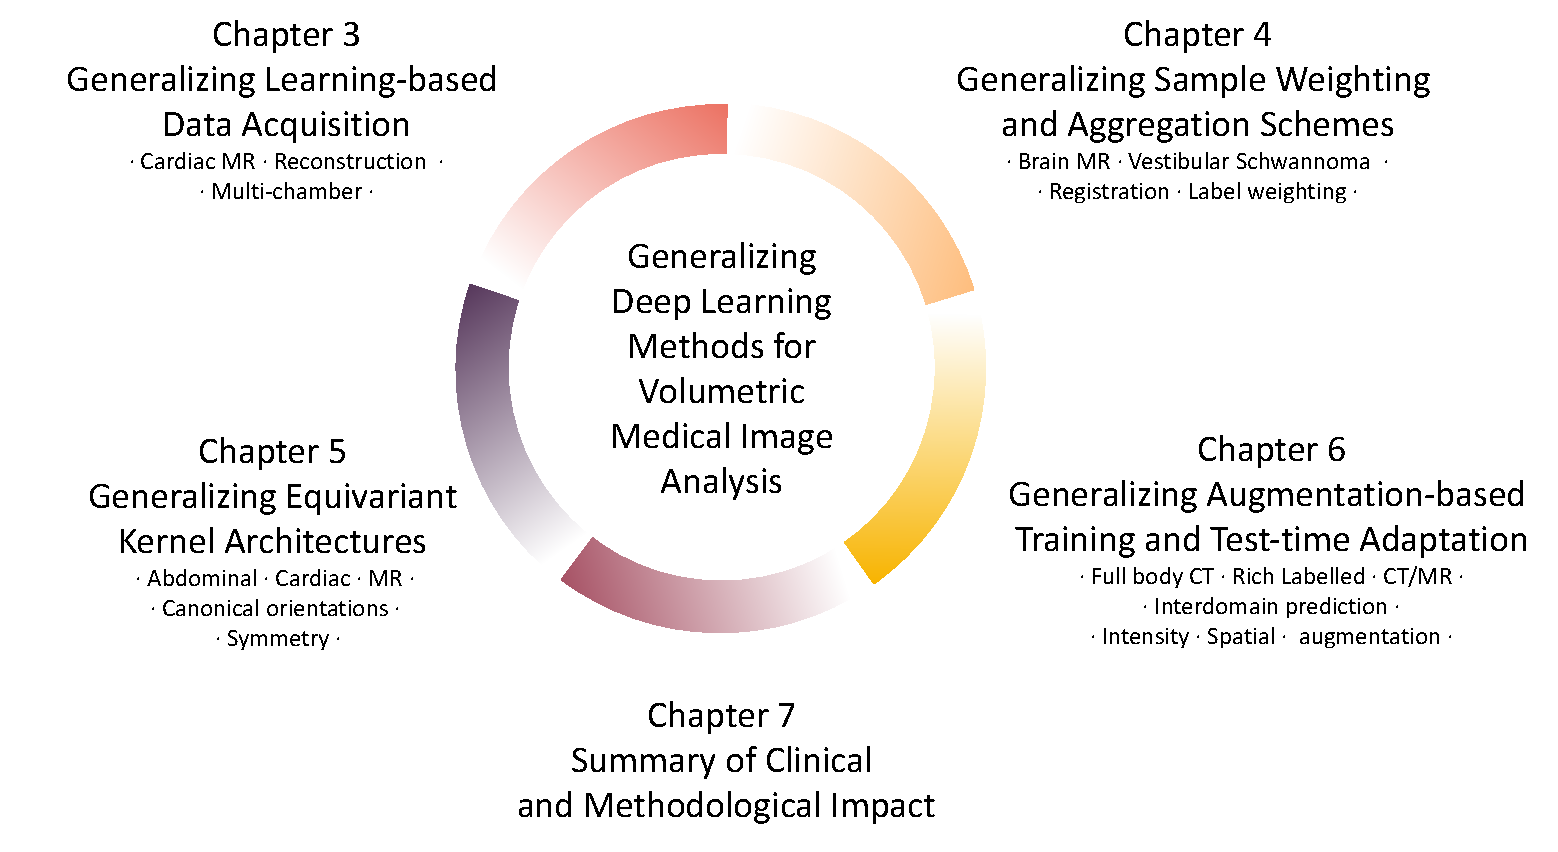
\includegraphics[width=\textwidth]{sections/01_introduction/figures/draft.pdf}
        \caption{Thesis draft}

    \end{figure}